\chapter{Index Analysis of the MNA}

der ane satz do + proof hopefully

seite 22 kap 7 netw top and dae ind for rlc - modelling and discretization circ prob

In the previous chapter we have seen two different kinds of Index concepts for differential algebraic equations. We have also seen that these two, even thoough they describe rather different structural aspects of the equation, are the same for our use-cases. This of course leads to the question : ´´What are the indices we can usually expect for MNA?''.

This chapter aims to answer that question for the linear RLC case. Which means that the RLC components are described by linear functions with positive capacitances, inductances and resistances. Thus the matrices
\begin{displaymath}
	C:=\frac{\partial q_C(w)}{\partial w}, \quad L:=\frac{\partial \phi_L(w)}{\partial w}, \quad G:=\frac{\partial r(w)}{\partial w}
\end{displaymath}

are positive definite and symmetric.

The generalization of these results to the nonlinear case still relies on positive definiteness.

Recall that we consider the equations resulting from the analysis above. These equations are of the form \ref{DAE-const-coeff}
\begin{displaymath}
	A y'(t) + B y(t) = f(t).
\end{displaymath}

Specifically the obtained equations from the Modified Nodal Analysis \ref{MNA_Matrixform} are
\begin{displaymath}
	\begin{pmatrix}
		A_C C A_C^\top & 0 & 0 \\
		0 & L & 0 \\
		0 & 0 & 0
	\end{pmatrix}
	*
	\begin{pmatrix}
		\dot{u} \\
		\dot{i_L} \\
		\dot{i_V}
	\end{pmatrix}
	+
	\begin{pmatrix}
		A_R G A_R^\top & A_L & A_V \\
		-A_L^\top & 0 & 0 \\
		-A_V^\top & 0 & 0 ä
	\end{pmatrix}
	*
	\begin{pmatrix}
		u \\
		i_L \\
		i_V
	\end{pmatrix}
	=
	\begin{pmatrix}
		-A_I i_{src} \\
		0 \\
		-v_{src}
	\end{pmatrix}.
\end{displaymath}

\section{General Index analysis}

Assuming the system only contains linear elements or is linearized at an operating point in order to investigate the system behaviour then the corresponding network equation represents a DAE with constant coefficients \ref{DAE-const-coeff}. We will denote $x=(u, i_L, i_V)^\top$. The structure of the system is reliant on the matrix $B$, thus we consider

\begin{itemize}
	\item \textbf{ODE-case}: \newline
	The matrix $B$ is regular in \ref{DAE-const-coeff}. This is the case iff the circuit contains no voltage sources and there are no nodes which have no path to ground via capacitors. Then the system represents a linear-implicit system of ODEs and can be transformed into the explicit ODE sytstem
	\begin{displaymath}
		\dot{x}=B^{-1}(-Ax+f(t)).
	\end{displaymath}
	Thus we obtain an index of $0$.
		
	\item \textbf{DAE-case}:
	The matrix $B$ is singular in \ref{DAE-const-coeff}. This is the interesting case which we will analyse further.
\end{itemize}

reminder for the structure obtained in previous chapter
\begin{align*}
	u'(t) + Ru(t) &= s(t), \\
	Nv'(t) + v(t) &= q(t)
\end{align*}

We now consider the nilpotency index of the matrix $N$, as seen in the previous chapter, this index correlates to the differentiation as well as the perturbation index.

\begin{enumerate}
	\item index 1 case
	Because $N$ is nilpotent with nipotency index $\nu = 1$ it holds that $N^1 = 0$, thus the system transforms to
	\begin{align*}
		u'(t) + Ru(t) &= s(t), \\
		v(t) &= q(t).
	\end{align*}
	This means that the algebraic variables are given explicitly. Thus the system can be written in ODE form. (what properies does R have?)

	\item index $\geq$ 2 case
	
	results in the solution we derived in \ref{solution-to-transformed-DAE-const-coeff-part2}. The index of the MNA is the same as $ind(A,B)$, which denotes the nilpotency index of $N$ as we have seen in the previous analysis in chapter 3.
\end{enumerate}

continue herer with modelling book from bottom of page 20-21 (did that on 26.11)

an algebraic constraint has to be fulfilled by thesolution. case of index 1 this equation is given explicitly. for index geq 2 it is given implicitly (i need to show that somewhere) 

system is sensitive to perturbations - small input noise can have arbitrarily large derivatives (shows in formula above for z)

book says - no severe numerical problems with index 1. might show up for implicit algebraic constraint.  Hence implicit numerical integration schemes for stiff systems are feasable.

however sever numerical problems may arrise for index geq 2. hidden algebraic constraints can make problems.

index is called algebraic index? - elaborate maybe on that

put that one chapter up?

differentiation index - since numerical differentiation is an unstable procedure this index gives a measure for the numerical problems to be expected when solving such systems

perturbation index - derivatives of perturbations enter solution


\begin{figure}[H]
	\centering
	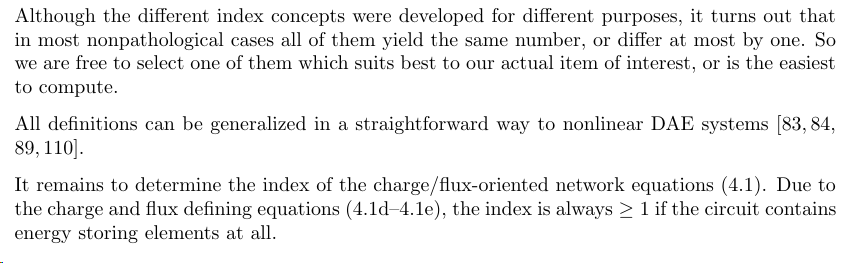
\includegraphics[width=0.7\linewidth]{screenshot022}
	\caption{}
	\label{fig:screenshot022}
\end{figure}


\section{Topological Conditions} 
reference to Tischendorf
basically chapter 7 of modelling book

From analyzing the MNA some conditions to the circuit topology can be obtained. We will be considering the impact of loops containing only capacitances and voltage sources as well as cutsets containing only inductances and current sources.

In \cite{Tischendorf2005Topological} they present very interesting results about the index of MNA equations. Namely the following:


\begin{theorem}[Index-1 condition] \cite{Tischendorf2004Topological}
	Let the matrices of the capacitances, inductances and resistances respectively be positive definite. If the network neither cointains \emph{inductance-current-source cutsets} nor (controlled?) \emph{capacitance-voltage-source loops}, then the MNA leads to an index-1 DAE.
\end{theorem}

\begin{theorem}[Index-2 condition] \cite{Tischendorf2004Topological}
	If the Network contains \emph{inductance-current-source cutsets} or \emph{capacitance-voltage-source loops} except for capacitance-only loops, then the MNA leads to an index-2 DAE.
\end{theorem}

These theorems can be interpreted as follows:


This means that for ´´reasonable'' RLC circuits (satisfying the prerequisites from the above theorems) the index will not exceed 2.


ker conditions from page 22

WE will apply those results to some examples: